\chapter{Observer Implications: Perception, Memory, and Mortality}

\section{Finite Observer}

We started with the assumption that observer exists as a finite informational structure, without any predefined
rules. Particulary, there is no rule stating that some abstract structures should play special role. In this view, to be and not to be
are like two sides of a coin - a mathematical binary objects. Head is equally probable as tail. So is empty set and any non-empty set.
So existence is inevitable.


There are infinitely many ways the finite information can encode that same functional structure called observer.
Some encodings are ultra-fine, massively redundant, hyper-detailed. Some are barely sufficient to sustain cognitive and biological processes of the observer.
Under a reasonable measure, overwhelmingly many realizations cluster near minimal sufficient encoding. And the most predictable, smooth
information compresses best. Therefore observer should expect to find themselves at that dominant most probable configuration, which are smooth and
predictable, just like the universe that we observe.


\section{The Observer in a Timeless Configuration Space}

The framework developed in the preceding chapters treats the universe as a static ensemble of informational configurations. At the foundational level, there is no global time parameter, no primitive dynamics, and no causal signal propagation. Past, present, and future do not exist as ontologically distinct regions; all configurations coexist timelessly.

This raises an immediate question: how can an observer perceive, remember, or experience anything at all in such a structure?

The resolution follows from the observer-conditioned probability measure. Observers do not receive information from an external world through causal transmission.
Instead, they are embedded within sequences of configurations that already encode all information they experience. Perception, memory, and temporal ordering are therefore
emergent properties of observer-compatible configuration sequences, not fundamental primitives.


\section{Perception Without Signal Transmission}

Within a static informational ensemble, no bits change because other bits change elsewhere. There is no metaphysical notion of a signal traveling from an object to an observer. Nevertheless, observers experience seeing, hearing, and sensing. Perception arises because observer-compatible configurations contain internally consistent correlations between observer states and environmental structure.
What is phenomenologically described as incoming sensory data is simply part of the observer’s informational configuration.

Seeing is not the reception of photons, hearing is not the reception of pressure waves, and sensation is not signal transmission.
These are stable relational patterns within dominant configurations. The observer experiences perception because the configurations in which it
exists already encode a coherent world that includes both the observer and its environment.


\section{Memory as an Execution Trace}

An observer is not a single configuration but a structured sequence of configurations. It can be viewed as an execution trace constrained by continuity conditions.
Memory is the internal encoding of this trace. The past corresponds to those portions of the execution trace already encoded within the observer’s internal state.
The future corresponds to the set of high-probability continuations compatible with observer integrity, compressibility, and survival.
As the observer progresses along a dominant walk through configuration space, memory grows monotonically.

This monotonic growth defines the experienced arrow of time. Time is therefore perspectival: it is not an external dimension but the ordinal ordering of observer-compatible configurations along a maximal-probability path.


\section{Observer Wavefunctions and Epistemic Closure}

For any observer, the total accessible information is finite and can be represented as a finite bitstring, or as a wavefunction defined over informational configurations.
This wavefunction admits many decompositions, but only a vanishingly small subset correspond to observers: coherent subsystems with sufficient structure to support memory, prediction, and internal consistency.
Crucially, an observer can only observe what its own wavefunction describes. Components outside this factorization carry negligible weight relative to the observer and cannot be integrated into memory or prediction.
What the observer calls the other observers, or the universe—are information encoded in the observers wavefunction.


\section{Interpolation, Extrapolation, and the Inside–Outside Distinction}

The wavefunction is not a physical field but an optimal spectral encoding of the observer’s information. Any finite history can be transformed into a spectral representation that
compresses large amounts of discrete data into a small number of coefficients. The dominance of wave-like descriptions arises because they are algorithmically cheaper than point-by-point encodings.

Interpolation corresponds to the reconstruction of configurations within the observer’s already-encoded execution trace. Because these data points are constrained by memory, the wavefunction is tightly pinned down. This produces the smooth, stable, and predictable laws of physics experienced locally. The interpolated region corresponds to what is phenomenologically described as the past or the inside.

Extrapolation occurs when the same spectral encoding is extended beyond the domain fixed by memory. In any complex-valued spectral model, extrapolation is inherently unstable. Small uncertainties in coefficients lead to rapidly diverging oscillations. When the observer wavefunction extrapolates toward unvisited configurations—interpreted as the distant future or the outside—its values grow extreme.

Planets, stars, and black holes are not fundamental objects but manifestations of this instability. They arise as large-amplitude fluctuations when a finite informational structure extrapolates beyond its constrained domain. 


\section{Entropy Gradients and Observer Self-Location}

Among all possible observer walks through configuration space, those that maximize compressibility dominate the observer-conditioned measure. These walks induce a perspectival arrow of time: an ordering from configurations with many compatible continuations to those with fewer.

The probability of emergent geometry and stable microstructure is not monotonic in entropy. At very low entropy, structure is absent and geometry collapses. At very high entropy, coherence dissolves. Rich, persistent structures dominate only at intermediate entropy.

Observers necessarily find themselves on one side of this entropy peak. Their perceived universe is determined by this self-location.

An observer located on the low-entropy side of the entropy profile experiences successive configurations of increasing entropy and differentiation. The perceived universe expands, a singularity appears in the past, and objects emerge irreversibly. This corresponds to what is traditionally described as a Big Bang.

An observer located on the high-entropy side experiences decreasing entropy and tightening constraints. The perceived universe collapses, a singularity appears in the future, and objects fall inward without escape. This corresponds to a black hole.

These are not distinct universes. They are different readings of the same timeless informational structure. Expansion and collapse are epistemic interpretations induced by observer self-location.


\section{Mortality as Vanishing Measure}

Geometric space gives the obserer a good sense over its information boundaries to increase the probability of surival. As an observer accumulates memory wavefunctions inevitably overlap at small scales (radiation etc.)
internal informational complexity increases. Initially this enhances survival by enabling better prediction and stability. However, increasing complexity reduces compressibility and narrows the set of
compatible continuations. Eventually, no high-probability continuations remain. The observer ceases to exist not through physical destruction but through vanishing measure.
Death is therefore a statistical event: the exhaustion of observer-compatible configurations.



\section{Conclusion}

The observer finds itself within configurations that already contain the universe, including other observers.
In this sense, we are not located inside the universe. The universe, as experienced, is encoded within us.

\begin{figure}[h]
    \centering
    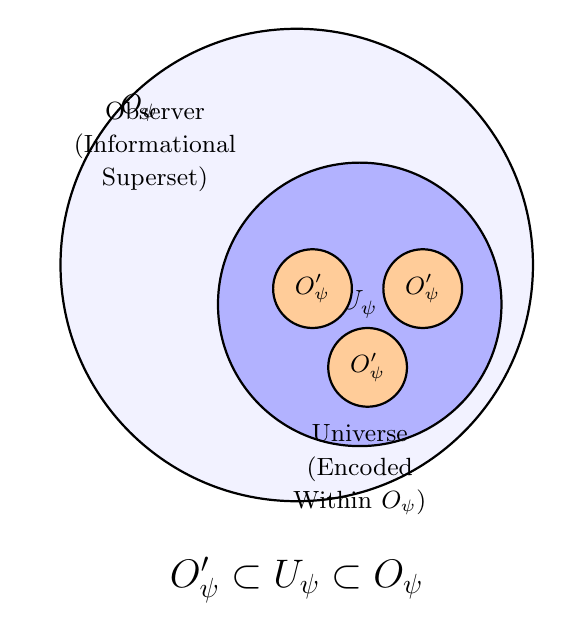
\begin{tikzpicture}
        % Observer O_\psi (Superset)
        \draw[thick, fill=blue!5] (0,0) circle (3cm);
        \node at (-2,2) {\textbf{$O_{\psi}$}};
        \node[text width=3cm, align=center] at (-1.8,1.5)
            {\small Observer\\(Informational Superset)};

        % Universe U_\psi (Encoded Subset)
        \draw[thick, fill=blue!30] (0.8,-0.5) circle (1.8cm);
        \node at (0.8,-0.5) {\textbf{$U_{\psi}$}};
        \node[text width=3cm, align=center] at (0.8,-2.6)
            {\small Universe\\(Encoded Within $O_{\psi}$)};

        % Other Observers O'_\psi
        \draw[thick, fill=orange!40] (0.2,-0.3) circle (0.5cm);
        \node at (0.2,-0.3) {\small \textbf{$O'_{\psi}$}};

        \draw[thick, fill=orange!40] (1.6,-0.3) circle (0.5cm);
        \node at (1.6,-0.3) {\small \textbf{$O'_{\psi}$}};

        \draw[thick, fill=orange!40] (0.9,-1.3) circle (0.5cm);
        \node at (0.9,-1.3) {\small \textbf{$O'_{\psi}$}};

        % Set relation
        \node at (0,-4) {\Large $O'_{\psi} \subset U_{\psi} \subset O_{\psi}$};
    \end{tikzpicture}
    \caption{Wavefunction-indexed encoding: the universe and other observers exist only as structures within the observer’s wavefunction.}
\end{figure}
